%----------------------------------------------------------------------------------------
%    PACKAGES AND THEMES
%----------------------------------------------------------------------------------------
\documentclass[aspectratio=169,xcolor=dvipsnames]{beamer}
\makeatletter
\def\input@path{{../BeamerTemplate/theme/}}
\makeatother
\usetheme{CleanEasy}
\usepackage[utf8]{inputenc}
\usepackage{lmodern}
\usepackage[T1]{fontenc}
\usepackage{fix-cm}
\usepackage{amsmath}
\usepackage{mathtools}
\usepackage{listings}
\usepackage{xcolor}
\usepackage{hyperref}
\usepackage{graphicx}
\usepackage{booktabs}
\usepackage{tikz}
\usetikzlibrary{positioning, shapes, arrows, calc, decorations.pathreplacing, arrows.meta, backgrounds, patterns, overlay-beamer-styles}
\usepackage{etoolbox}
\usepackage{animate}

%----------------------------------------------------------------------------------------
%    LAYOUT CONFIGURATION
%----------------------------------------------------------------------------------------
\input{../BeamerTemplate/configs/configs}

%----------------------------------------------------------------------------------------
%    TITLE PAGE CONFIGURATION
%----------------------------------------------------------------------------------------
\title[Arrays]{Data Structures: Arrays}
\author{Data Structure Course}
\institute{DGIST}
\date{\today}

% Simple title page without logos
\titlegraphic{}

%----------------------------------------------------------------------------------------

\begin{document}

\begin{frame}[plain]
  \titlepage
\end{frame}

\begin{frame}[plain]{Contents}
  \tableofcontents
\end{frame}

%----------------------------------------------------------------------------------------
%    INTRODUCTION
%----------------------------------------------------------------------------------------
\section{Introduction to Arrays}

\begin{frame}{What is an Array?}
  \begin{definition}
    An \textbf{array} is a contiguous memory block that stores elements of the same type, supporting \textbf{O(1) indexing}.
  \end{definition}

  \vspace{0.5cm}

  \begin{columns}
    \begin{column}{0.6\textwidth}
      Key characteristics:
      \begin{itemize}
        \item Fixed or dynamic size
        \item Elements stored consecutively in memory
        \item Direct access via index
        \item Cache-friendly data structure
        \item Foundation for many other data structures
      \end{itemize}
    \end{column}
    \begin{column}{0.35\textwidth}
      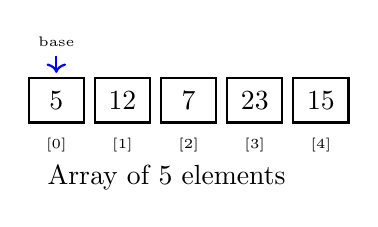
\begin{tikzpicture}[scale=0.7]
        % Array visualization
        \foreach \i/\val in {0/5, 1/12, 2/7, 3/23, 4/15} {
          \draw[thick] (\i*1.2,0) rectangle (\i*1.2+1,0.8);
          \node at (\i*1.2+0.5,0.4) {\val};
          \node[below] at (\i*1.2+0.5,-0.1) {\tiny[\i]};
        }

        \node[below] at (2.5,-0.6) {Array of 5 elements};

        % Memory address indicator
        \draw[->, thick, blue] (0.5,1.2) -- (0.5,0.9);
        \node[above] at (0.5,1.2) {\tiny base};
      \end{tikzpicture}
    \end{column}
  \end{columns}

  \vspace{0.3cm}

  \begin{alertblock}{Memory Address Calculation}
    Address of \texttt{arr[i]} = \texttt{base\_address + i × sizeof(element)}
  \end{alertblock}
\end{frame}

%----------------------------------------------------------------------------------------
%    STATIC VS DYNAMIC ARRAYS
%----------------------------------------------------------------------------------------
\section{Static vs Dynamic Arrays}

\begin{frame}[fragile]{Static Arrays}
  \begin{block}{Definition}
    Fixed size determined at compile time or initialization
  \end{block}

  \begin{columns}
    \begin{column}{0.48\textwidth}
      \textbf{Advantages:}
      \begin{itemize}
        \item No resize overhead
        \item Predictable memory usage
        \item Slightly faster access
        \item Simple memory management
      \end{itemize}

      \vspace{0.3cm}

      \textbf{Disadvantages:}
      \begin{itemize}
        \item Cannot grow or shrink
        \item Must know size in advance
        \item Wasted space if overallocated
        \item Insufficient space if underallocated
      \end{itemize}
    \end{column}
    \begin{column}{0.48\textwidth}
      \begin{exampleblock}{Examples}
        \textbf{C:}
        \begin{lstlisting}[language=C,basicstyle=\tiny\ttfamily]
int arr[100];  // Fixed size
        \end{lstlisting}

        \textbf{Java:}
        \begin{lstlisting}[language=Java,basicstyle=\tiny\ttfamily]
int[] arr = new int[100];
        \end{lstlisting}

        \textbf{C++:}
        \begin{lstlisting}[language=C++,basicstyle=\tiny\ttfamily]
int arr[100];
std::array<int, 100> arr;
        \end{lstlisting}
      \end{exampleblock}

      \vspace{0.2cm}

      \begin{alertblock}{Use Case}
        When size is known and fixed (e.g., days of week, fixed buffers)
      \end{alertblock}
    \end{column}
  \end{columns}
\end{frame}

\begin{frame}[fragile]{Dynamic Arrays}
  \begin{block}{Definition}
    Resizable arrays that grow as needed
  \end{block}

  \begin{columns}
    \begin{column}{0.55\textwidth}
      \textbf{Growth Strategy:}
      \begin{itemize}
        \item Start with small capacity
        \item Double capacity when full (typical)
        \item Allocate new array and copy elements
        \item Free old array
      \end{itemize}

      \vspace{0.3cm}

      \textbf{Examples:}
      \begin{itemize}
        \item C++: \texttt{std::vector}
        \item Java: \texttt{ArrayList}
        \item Python: \texttt{list}
        \item C\#: \texttt{List<T>}
      \end{itemize}
    \end{column}
    \begin{column}{0.4\textwidth}
      \begin{exampleblock}{Python Implementation}
        \begin{lstlisting}[language=Python,basicstyle=\tiny\ttfamily]
class DynamicArray:
    def __init__(self):
        self.capacity = 1
        self.size = 0
        self.array = [None] * self.capacity

    def append(self, item):
        if self.size == self.capacity:
            self._resize()
        self.array[self.size] = item
        self.size += 1

    def _resize(self):
        self.capacity *= 2
        new_array = [None] * self.capacity
        for i in range(self.size):
            new_array[i] = self.array[i]
        self.array = new_array
        \end{lstlisting}
      \end{exampleblock}
    \end{column}
  \end{columns}
\end{frame}

\begin{frame}{Comparison: Static vs Dynamic Arrays}
  \begin{center}
    \begin{tabular}{l|c|c}
      \toprule
      \textbf{Operation} & \textbf{Static Array} & \textbf{Dynamic Array} \\
      \midrule
      Access & O(1) & O(1) \\
      Append & N/A & O(1) amortized \\
      Insert (middle) & O(n) & O(n) \\
      Delete (middle) & O(n) & O(n) \\
      Memory & Exact & 1.5-2× actual size \\
      Resize & No & Yes (expensive) \\
      \bottomrule
    \end{tabular}
  \end{center}

  \vspace{0.5cm}

  \begin{columns}
    \begin{column}{0.48\textwidth}
      \begin{block}{Static Arrays Best For}
        \begin{itemize}
          \item Fixed-size data
          \item Memory-constrained systems
          \item Real-time systems
        \end{itemize}
      \end{block}
    \end{column}
    \begin{column}{0.48\textwidth}
      \begin{block}{Dynamic Arrays Best For}
        \begin{itemize}
          \item Unknown or changing size
          \item Frequent additions
          \item General-purpose use
        \end{itemize}
      \end{block}
    \end{column}
  \end{columns}
\end{frame}

%----------------------------------------------------------------------------------------
%    AMORTIZED ANALYSIS
%----------------------------------------------------------------------------------------
\section{Amortized Analysis}

\begin{frame}{Dynamic Array Resizing Cost}
  \begin{block}{Resizing Strategy}
    When array is full, allocate new array with 2× capacity
  \end{block}

  \vspace{0.3cm}

  \begin{columns}
    \begin{column}{0.55\textwidth}
      \textbf{Single Resize Cost: O(n)}
      \begin{itemize}
        \item Allocate new array: O(capacity)
        \item Copy all n elements: O(n)
        \item Free old array: O(1)
      \end{itemize}

      \vspace{0.3cm}

      \textbf{But resizes are infrequent!}
      \begin{itemize}
        \item Resizes at sizes: 1, 2, 4, 8, 16, ..., n
        \item Total resizes: $\log_2 n$
        \item Total copy cost: $1 + 2 + 4 + ... + n = 2n - 1$
      \end{itemize}
    \end{column}
    \begin{column}{0.4\textwidth}
      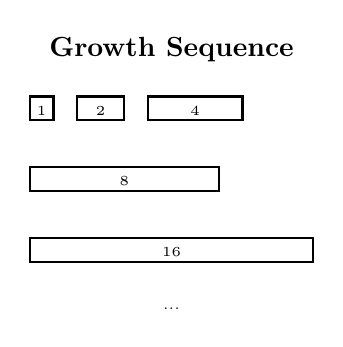
\begin{tikzpicture}[scale=0.6]
        % Visualization of growth
        \node at (3,6) {\textbf{Growth Sequence}};

        \draw[thick] (0,4.5) rectangle (0.5,5);
        \node at (0.25,4.7) {\tiny 1};

        \draw[thick] (1,4.5) rectangle (2,5);
        \node at (1.5,4.7) {\tiny 2};

        \draw[thick] (2.5,4.5) rectangle (4.5,5);
        \node at (3.5,4.7) {\tiny 4};

        \draw[thick] (0,3) rectangle (4,3.5);
        \node at (2,3.2) {\tiny 8};

        \draw[thick] (0,1.5) rectangle (6,2);
        \node at (3,1.7) {\tiny 16};

        \node at (3,0.5) {\tiny ...};
      \end{tikzpicture}
    \end{column}
  \end{columns}

  \vspace{0.3cm}

  \begin{exampleblock}{Amortized Analysis Result}
    Average cost per insertion: $\frac{O(n)}{n} = \textbf{O(1) amortized}$
  \end{exampleblock}
\end{frame}

\begin{frame}{Accounting Method for Amortized Analysis}
  \begin{block}{Intuition}
    Charge extra "credits" for cheap operations to pay for expensive ones
  \end{block}

  \vspace{0.3cm}

  \begin{columns}
    \begin{column}{0.5\textwidth}
      \textbf{Charge \$3 per insertion:}
      \begin{itemize}
        \item \$1 for actual insertion
        \item \$2 saved as credit for future resize
      \end{itemize}

      \vspace{0.3cm}

      \textbf{When resize happens:}
      \begin{itemize}
        \item Need to copy n elements
        \item Each element has \$2 credit saved
        \item Total credits: \$2n
        \item Resize cost: \$n (copying)
        \item Credits cover the cost!
      \end{itemize}
    \end{column}
    \begin{column}{0.45\textwidth}
      \begin{exampleblock}{Growth Factor Comparison}
        \begin{tabular}{c|c|c}
          \textbf{Factor} & \textbf{Memory} & \textbf{Frequency} \\
          \hline
          1.5× & Lower & More \\
          2× & Higher & Less \\
        \end{tabular}
      \end{exampleblock}

      \vspace{0.3cm}

      \begin{alertblock}{Shrinking Strategy}
        Shrink when \texttt{size < capacity/4} \\
        (not \texttt{capacity/2} to avoid thrashing)
      \end{alertblock}
    \end{column}
  \end{columns}

  \vspace{0.3cm}

  \begin{center}
    \textbf{Trade-off:} Space efficiency vs resize frequency
  \end{center}
\end{frame}

%----------------------------------------------------------------------------------------
%    ARRAY OPERATIONS
%----------------------------------------------------------------------------------------
\section{Array Operations}

\begin{frame}[fragile]{Access and Search Operations}
  \begin{columns}
    \begin{column}{0.48\textwidth}
      \begin{block}{Access by Index: O(1)}
        \begin{lstlisting}[language=Python,basicstyle=\small\ttfamily]
element = arr[i]
        \end{lstlisting}
        Direct memory calculation: \\
        \texttt{base + i × sizeof(element)}
      \end{block}

      \vspace{0.3cm}

      \begin{block}{Linear Search: O(n)}
        \begin{lstlisting}[language=Python,basicstyle=\tiny\ttfamily]
def linear_search(arr, target):
    for i in range(len(arr)):
        if arr[i] == target:
            return i
    return -1
        \end{lstlisting}
        Check each element sequentially
      \end{block}
    \end{column}
    \begin{column}{0.48\textwidth}
      \begin{block}{Binary Search: O(log n)}
        \textbf{Only for sorted arrays!}
        \begin{lstlisting}[language=Python,basicstyle=\tiny\ttfamily]
def binary_search(arr, target):
    left, right = 0, len(arr) - 1
    while left <= right:
        mid = left + (right - left) // 2
        if arr[mid] == target:
            return mid
        elif arr[mid] < target:
            left = mid + 1
        else:
            right = mid - 1
    return -1
        \end{lstlisting}
      \end{block}

      \vspace{0.2cm}

      \begin{alertblock}{Key Insight}
        Binary search eliminates half the search space each iteration
      \end{alertblock}
    \end{column}
  \end{columns}
\end{frame}

\begin{frame}[fragile]{Insert and Delete Operations}
  \begin{columns}
    \begin{column}{0.48\textwidth}
      \begin{block}{Insert at Position i: O(n)}
        \begin{lstlisting}[language=Python,basicstyle=\tiny\ttfamily]
def insert(arr, index, value):
    arr.append(None)  # Ensure space
    # Shift elements right
    for i in range(len(arr)-1, index, -1):
        arr[i] = arr[i-1]
    arr[index] = value
        \end{lstlisting}
      \end{block}

      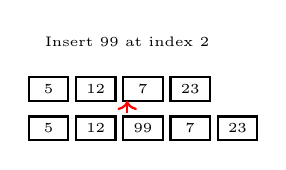
\begin{tikzpicture}[scale=0.5]
        \node at (2.5,2.5) {\tiny Insert 99 at index 2};

        % Before
        \foreach \i/\val in {0/5, 1/12, 2/7, 3/23} {
          \draw[thick] (\i*1.2,1) rectangle (\i*1.2+1,1.6);
          \node at (\i*1.2+0.5,1.3) {\tiny\val};
        }

        % After
        \foreach \i/\val in {0/5, 1/12, 2/99, 3/7, 4/23} {
          \draw[thick] (\i*1.2,0) rectangle (\i*1.2+1,0.6);
          \node at (\i*1.2+0.5,0.3) {\tiny\val};
        }

        \draw[->, thick, red] (2.5,0.7) -- (2.5,1);
      \end{tikzpicture}
    \end{column}
    \begin{column}{0.48\textwidth}
      \begin{block}{Delete at Position i: O(n)}
        \begin{lstlisting}[language=Python,basicstyle=\tiny\ttfamily]
def delete(arr, index):
    # Shift elements left
    for i in range(index, len(arr)-1):
        arr[i] = arr[i+1]
    arr.pop()  # Remove last
        \end{lstlisting}
      \end{block}

      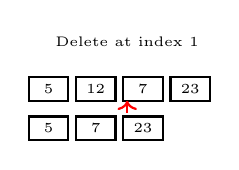
\begin{tikzpicture}[scale=0.5]
        \node at (2.5,2.5) {\tiny Delete at index 1};

        % Before
        \foreach \i/\val in {0/5, 1/12, 2/7, 3/23} {
          \draw[thick] (\i*1.2,1) rectangle (\i*1.2+1,1.6);
          \node at (\i*1.2+0.5,1.3) {\tiny\val};
        }

        % After
        \foreach \i/\val in {0/5, 1/7, 2/23} {
          \draw[thick] (\i*1.2,0) rectangle (\i*1.2+1,0.6);
          \node at (\i*1.2+0.5,0.3) {\tiny\val};
        }

        \draw[->, thick, red] (2.5,0.7) -- (2.5,1);
      \end{tikzpicture}
    \end{column}
  \end{columns}

  \vspace{0.3cm}

  \begin{alertblock}{Performance Summary}
    \begin{itemize}
      \item Insert/delete at end: O(1) amortized
      \item Insert/delete at beginning: O(n) - worst case
      \item Insert/delete in middle: O(n) - must shift elements
    \end{itemize}
  \end{alertblock}
\end{frame}

%----------------------------------------------------------------------------------------
%    MULTIDIMENSIONAL ARRAYS
%----------------------------------------------------------------------------------------
\section{Multidimensional Arrays}

\begin{frame}[fragile]{2D Arrays (Matrices)}
  \begin{columns}
    \begin{column}{0.5\textwidth}
      \begin{exampleblock}{Declaration}
        \textbf{Python:}
        \begin{lstlisting}[language=Python,basicstyle=\tiny\ttfamily]
matrix = [[0]*cols for _ in range(rows)]
        \end{lstlisting}

        \textbf{Java:}
        \begin{lstlisting}[language=Java,basicstyle=\tiny\ttfamily]
int[][] matrix = new int[rows][cols];
        \end{lstlisting}

        \textbf{C++:}
        \begin{lstlisting}[language=C++,basicstyle=\tiny\ttfamily]
vector<vector<int>> matrix(rows,
    vector<int>(cols));
        \end{lstlisting}
      \end{exampleblock}

      \vspace{0.2cm}

      \begin{block}{Accessing Elements}
        \texttt{element = matrix[i][j]}

        Time: O(1)
      \end{block}
    \end{column}
    \begin{column}{0.45\textwidth}
      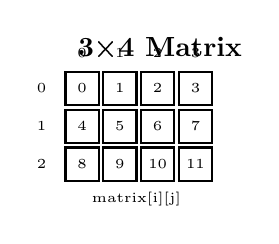
\begin{tikzpicture}[scale=0.6]
        \node at (2,3.5) {\textbf{3×4 Matrix}};

        % Draw matrix
        \foreach \i in {0,1,2} {
          \foreach \j in {0,1,2,3} {
            \draw[thick] (\j*0.8,3-\i*0.8) rectangle (\j*0.8+0.7,3-\i*0.8-0.7);
            \pgfmathtruncatemacro{\val}{\i*4+\j}
            \node at (\j*0.8+0.35,3-\i*0.8-0.35) {\tiny\val};
          }
        }

        % Indices
        \node[left] at (-0.2,2.65) {\tiny 0};
        \node[left] at (-0.2,1.85) {\tiny 1};
        \node[left] at (-0.2,1.05) {\tiny 2};

        \node[above] at (0.35,3.1) {\tiny 0};
        \node[above] at (1.15,3.1) {\tiny 1};
        \node[above] at (1.95,3.1) {\tiny 2};
        \node[above] at (2.75,3.1) {\tiny 3};

        \node at (1.5,0.3) {\tiny matrix[i][j]};
      \end{tikzpicture}
    \end{column}
  \end{columns}
\end{frame}

\begin{frame}{Memory Layout: Row-Major vs Column-Major}
  \begin{columns}
    \begin{column}{0.48\textwidth}
      \begin{block}{Row-Major Order}
        Used in: C, C++, Python, Java

        \vspace{0.2cm}

        Store rows contiguously: \\
        \texttt{[row0][row1][row2]...}

        \vspace{0.2cm}

        \textbf{Address calculation:} \\
        \texttt{base + (i × cols + j) × size}

        \vspace{0.2cm}

        \textbf{Better for:}
        \begin{itemize}
          \item Iterating by rows
          \item Row-wise operations
        \end{itemize}
      \end{block}
    \end{column}
    \begin{column}{0.48\textwidth}
      \begin{block}{Column-Major Order}
        Used in: Fortran, MATLAB

        \vspace{0.2cm}

        Store columns contiguously: \\
        \texttt{[col0][col1][col2]...}

        \vspace{0.2cm}

        \textbf{Address calculation:} \\
        \texttt{base + (j × rows + i) × size}

        \vspace{0.2cm}

        \textbf{Better for:}
        \begin{itemize}
          \item Iterating by columns
          \item Column-wise operations
        \end{itemize}
      \end{block}
    \end{column}
  \end{columns}

  \vspace{0.3cm}

  \begin{alertblock}{Performance Impact}
    Accessing memory in the wrong order can cause 10-100× slowdown due to cache misses!
  \end{alertblock}
\end{frame}

\begin{frame}[fragile]{Common Matrix Operations}
  \begin{columns}
    \begin{column}{0.48\textwidth}
      \begin{block}{Transpose: O(rows × cols)}
        \begin{lstlisting}[language=Python,basicstyle=\tiny\ttfamily]
def transpose(matrix):
    rows = len(matrix)
    cols = len(matrix[0])
    result = [[0]*rows for _ in range(cols)]
    for i in range(rows):
        for j in range(cols):
            result[j][i] = matrix[i][j]
    return result
        \end{lstlisting}
      \end{block}

      \vspace{0.2cm}

      \begin{exampleblock}{Example}
        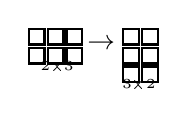
\begin{tikzpicture}[scale=0.4]
          % Original
          \foreach \i in {0,1} {
            \foreach \j in {0,1,2} {
              \draw[thick] (\j*0.6,-\i*0.6) rectangle (\j*0.6+0.5,-\i*0.6-0.5);
            }
          }
          \node at (0.9,-1.2) {\tiny 2×3};

          \node at (2.3,-0.5) {$\rightarrow$};

          % Transposed
          \foreach \i in {0,1,2} {
            \foreach \j in {0,1} {
              \draw[thick] (3+\j*0.6,-\i*0.6) rectangle (3+\j*0.6+0.5,-\i*0.6-0.5);
            }
          }
          \node at (3.5,-1.8) {\tiny 3×2};
        \end{tikzpicture}
      \end{exampleblock}
    \end{column}
    \begin{column}{0.48\textwidth}
      \begin{block}{Rotate 90° Clockwise}
        \begin{lstlisting}[language=Python,basicstyle=\tiny\ttfamily,escapechar=@]
def rotate_90(matrix):
    n = len(matrix)
    # 1. Transpose
    for i in range(n):
        for j in range(i, n):
            temp = matrix[i][j]
            matrix[i][j] = matrix[j][i]
            matrix[j][i] = temp

    # 2. Reverse each row
    for i in range(n):
        matrix[i].reverse()
        \end{lstlisting}
      \end{block}

      \vspace{0.2cm}

      \begin{block}{Matrix Multiplication}
        \textbf{Naive:} O(n³) \\
        \textbf{Strassen:} O(n$^{2.37}$) \\
        \textbf{Coppersmith-Winograd:} O(n$^{2.376}$)
      \end{block}
    \end{column}
  \end{columns}
\end{frame}

%----------------------------------------------------------------------------------------
%    MEMORY AND CACHE
%----------------------------------------------------------------------------------------
\section{Memory Layout \& Cache Locality}

\begin{frame}{Cache Hierarchy and Performance}
  \begin{columns}
    \begin{column}{0.5\textwidth}
      \begin{block}{Memory Hierarchy}
        \begin{tabular}{l|c|c}
          \textbf{Level} & \textbf{Size} & \textbf{Latency} \\
          \hline
          L1 Cache & 32-64 KB & 1-4 cycles \\
          L2 Cache & 256 KB-1 MB & 10-20 cycles \\
          L3 Cache & 8-32 MB & 40-75 cycles \\
          RAM & GB & 200+ cycles \\
        \end{tabular}
      \end{block}

      \vspace{0.3cm}

      \begin{block}{Cache Line}
        \begin{itemize}
          \item Typical size: 64 bytes
          \item Fetching one element loads entire cache line
          \item Sequential access benefits from prefetching
        \end{itemize}
      \end{block}
    \end{column}
    \begin{column}{0.45\textwidth}
      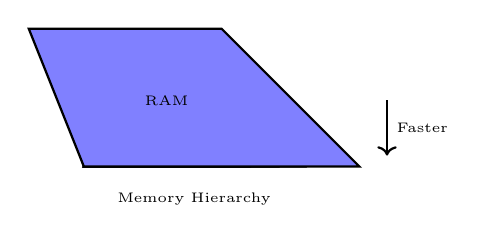
\begin{tikzpicture}[scale=0.7]
        % Memory hierarchy pyramid
        \draw[thick, fill=blue!20] (0,0) -- (3,0) -- (2.5,0.8) -- (0.5,0.8) -- cycle;
        \node at (1.5,0.4) {\tiny L1 Cache};

        \draw[thick, fill=blue!30] (0,0) -- (3.5,0) -- (2.5,0.8) -- (0.5,0.8) -- cycle;
        \node at (1.5,0.3) {\tiny L2 Cache};

        \draw[thick, fill=blue!40] (0,0) -- (4,0) -- (2.5,1.5) -- (-0.5,1.5) -- cycle;
        \node at (1.5,0.7) {\tiny L3 Cache};

        \draw[thick, fill=blue!50] (0,0) -- (5,0) -- (2.5,2.5) -- (-1,2.5) -- cycle;
        \node at (1.5,1.2) {\tiny RAM};

        \draw[->, thick] (5.5,1.2) -- (5.5,0.2);
        \node[right] at (5.5,0.7) {\tiny Faster};

        \node[below] at (2,-0.3) {\tiny Memory Hierarchy};
      \end{tikzpicture}
    \end{column}
  \end{columns}

  \vspace{0.3cm}

  \begin{alertblock}{Key Insight}
    Accessing data in cache vs RAM can be 100-200× faster!
  \end{alertblock}
\end{frame}

\begin{frame}[fragile]{Spatial Locality: Good vs Bad Access Patterns}
  \begin{columns}
    \begin{column}{0.48\textwidth}
      \begin{exampleblock}{Good: Sequential Access}
        \begin{lstlisting}[language=Python,basicstyle=\small\ttfamily]
# Excellent cache locality
sum = 0
for i in range(n):
    sum += arr[i]
        \end{lstlisting}

        \vspace{0.2cm}

        \begin{itemize}
          \item Accesses consecutive memory
          \item Cache prefetching works well
          \item Minimizes cache misses
        \end{itemize}
      \end{exampleblock}
    \end{column}
    \begin{column}{0.48\textwidth}
      \begin{alertblock}{Bad: Random Access}
        \begin{lstlisting}[language=Python,basicstyle=\small\ttfamily]
# Poor cache locality
sum = 0
for i in random_indices:
    sum += arr[i]
        \end{lstlisting}

        \vspace{0.2cm}

        \begin{itemize}
          \item Jumps around memory
          \item No benefit from prefetching
          \item Frequent cache misses
        \end{itemize}
      \end{alertblock}
    \end{column}
  \end{columns}

  \vspace{0.5cm}

  \begin{block}{Matrix Traversal Example (C/C++ row-major)}
    \begin{lstlisting}[language=C++,basicstyle=\tiny\ttfamily]
// GOOD: Row-wise iteration (follows memory layout)
for (int i = 0; i < rows; i++)
    for (int j = 0; j < cols; j++)
        sum += matrix[i][j];

// BAD: Column-wise iteration (jumps across cache lines)
for (int j = 0; j < cols; j++)
    for (int i = 0; i < rows; i++)
        sum += matrix[i][j];
    \end{lstlisting}
  \end{block}
\end{frame}

\begin{frame}[fragile]{Optimization: Array of Structures vs Structure of Arrays}
  \begin{columns}
    \begin{column}{0.48\textwidth}
      \begin{block}{Array of Structures (AoS)}
        \begin{lstlisting}[language=C++,basicstyle=\tiny\ttfamily]
struct Point {
    float x, y, z;
};
Point points[1000];

// Access x coordinates
for (int i = 0; i < 1000; i++)
    sum += points[i].x;
        \end{lstlisting}

        \vspace{0.2cm}

        \textbf{Memory layout:} \\
        \texttt{x0 y0 z0 | x1 y1 z1 | x2 y2 z2 ...}

        \vspace{0.2cm}

        \textbf{Issue:} Loading unnecessary y, z values
      \end{block}
    \end{column}
    \begin{column}{0.48\textwidth}
      \begin{block}{Structure of Arrays (SoA)}
        \begin{lstlisting}[language=C++,basicstyle=\tiny\ttfamily]
struct Points {
    float x[1000];
    float y[1000];
    float z[1000];
};
Points points;

// Access x coordinates
for (int i = 0; i < 1000; i++)
    sum += points.x[i];
        \end{lstlisting}

        \vspace{0.2cm}

        \textbf{Memory layout:} \\
        \texttt{x0 x1 x2 ... | y0 y1 y2 ... | z0 z1 z2 ...}

        \vspace{0.2cm}

        \textbf{Benefit:} Better cache locality for single field
      \end{block}
    \end{column}
  \end{columns}

  \vspace{0.3cm}

  \begin{exampleblock}{When to Use SoA}
    SIMD operations, GPU computing, frequently accessing single fields
  \end{exampleblock}
\end{frame}

%----------------------------------------------------------------------------------------
%    APPLICATIONS
%----------------------------------------------------------------------------------------
\section{Applications \& Limitations}

\begin{frame}{When to Use Arrays}
  \begin{columns}
    \begin{column}{0.48\textwidth}
      \begin{block}{Common Applications}
        \begin{itemize}
          \item \textbf{Lookup tables}: ASCII mappings, precomputed values
          \item \textbf{Buffers}: Fixed-size data storage, I/O buffers
          \item \textbf{Stacks/Queues}: Array-based implementations
          \item \textbf{Dynamic programming}: Memoization tables
          \item \textbf{Sorting algorithms}: In-place sorting
          \item \textbf{Image processing}: Pixel arrays (2D/3D)
          \item \textbf{Scientific computing}: Vectors, matrices, tensors
        \end{itemize}
      \end{block}
    \end{column}
    \begin{column}{0.48\textwidth}
      \begin{block}{Advantages}
        \begin{itemize}
          \item[$\checkmark$] O(1) random access by index
          \item[$\checkmark$] Cache-friendly (contiguous memory)
          \item[$\checkmark$] Simple and intuitive
          \item[$\checkmark$] Low memory overhead
          \item[$\checkmark$] Excellent for iteration
        \end{itemize}
      \end{block}

      \vspace{0.2cm}

      \begin{alertblock}{Limitations}
        \begin{itemize}
          \item[$\times$] Fixed size or resize overhead
          \item[$\times$] O(n) insertion/deletion in middle
          \item[$\times$] Wasted space if sparse
          \item[$\times$] Cannot efficiently grow in middle
        \end{itemize}
      \end{alertblock}
    \end{column}
  \end{columns}
\end{frame}

\begin{frame}{When to Use Alternatives}
  \begin{center}
    \begin{tabular}{p{4cm}|p{3.5cm}|p{3.5cm}}
      \toprule
      \textbf{Use Case} & \textbf{Better Alternative} & \textbf{Reason} \\
      \midrule
      Frequent insertions/deletions & Linked List & O(1) insert/delete \\
      \midrule
      Unknown size, many insertions & Dynamic Array & Amortized O(1) append \\
      \midrule
      Key-value lookups & Hash Table & O(1) average lookup \\
      \midrule
      Sorted data with insertions & Binary Search Tree & O(log n) operations \\
      \midrule
      Priority queue & Heap & O(log n) insert/extract-min \\
      \midrule
      Sparse data & Hash Table / Sparse Matrix & Space efficient \\
      \bottomrule
    \end{tabular}
  \end{center}

  \vspace{0.5cm}

  \begin{exampleblock}{Real-World Examples}
    \textbf{ArrayList} (Java), \textbf{std::vector} (C++), \textbf{NumPy arrays} (Python), \textbf{Circular buffer}, \textbf{Bitmap}
  \end{exampleblock}
\end{frame}

%----------------------------------------------------------------------------------------
%    SUMMARY
%----------------------------------------------------------------------------------------
\section{Summary}

\begin{frame}{Key Takeaways}
  \begin{block}{Array Fundamentals}
    \begin{itemize}
      \item Contiguous memory blocks with O(1) indexing
      \item Foundation for many data structures
      \item Direct memory address calculation
    \end{itemize}
  \end{block}

  \begin{block}{Static vs Dynamic}
    \begin{itemize}
      \item Static: fixed size, no overhead, predictable
      \item Dynamic: resizable, O(1) amortized append, flexible
      \item Amortized analysis shows O(1) average cost for dynamic growth
    \end{itemize}
  \end{block}

  \begin{block}{Performance Considerations}
    \begin{itemize}
      \item Cache locality is critical: 10-100× performance difference
      \item Access patterns matter: sequential > random
      \item Row-major vs column-major order affects cache performance
      \item Consider SoA vs AoS for specific access patterns
    \end{itemize}
  \end{block}

  \begin{block}{When to Use}
    \begin{itemize}
      \item Best for: random access, iteration, fixed/predictable size
      \item Avoid for: frequent insertions/deletions, unknown size, sparse data
    \end{itemize}
  \end{block}
\end{frame}

\begin{frame}[plain]
  \begin{center}
    {\Huge Thank You!}

    \vspace{1cm}

    {\large Questions?}
  \end{center}
\end{frame}

\end{document}
